\section{Durchführung}
\label{sec:Durchführung}
Der grundlegende Versuchsaufbau ist in Abbildung \ref{fig:aufbau} zu sehen.

\begin{figure}
  \centering
  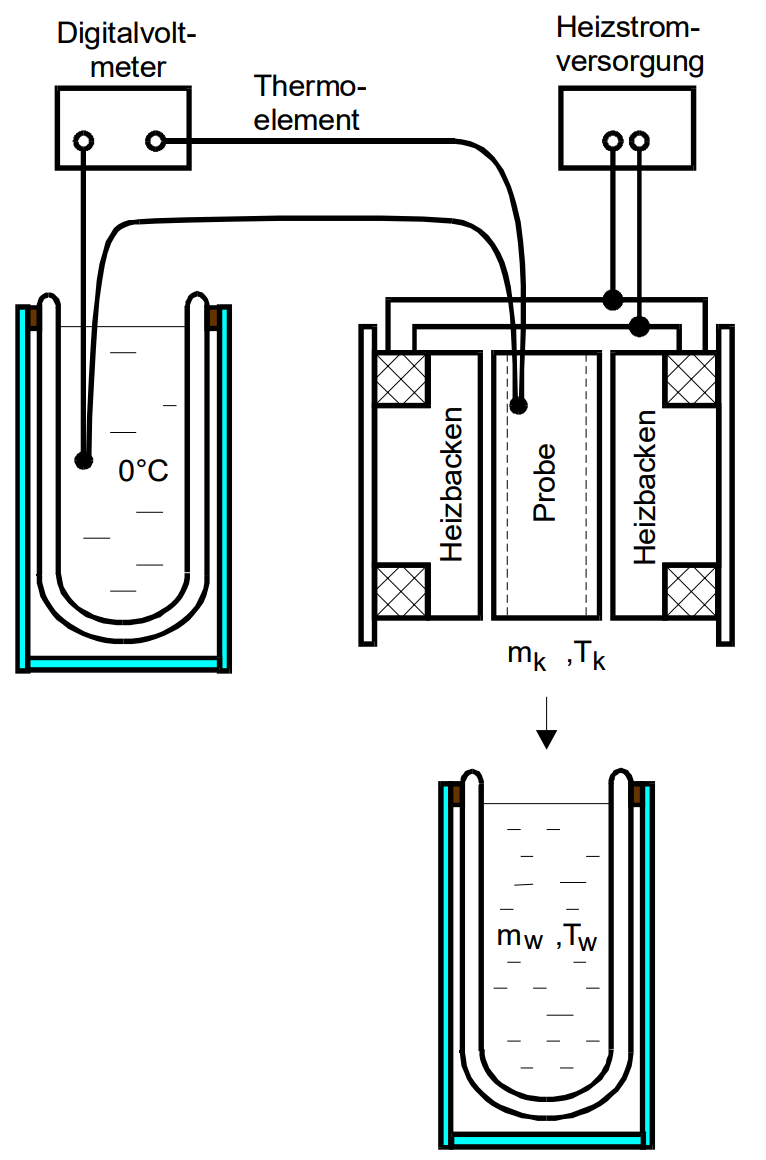
\includegraphics[width=300pt]{data/aufbau.png}
  \caption{Skizze des Versuchsaufbaus \cite{Versuchsanleitung}}
  \label{fig:aufbau}
\end{figure}

Der Versuch wird hier ohne Heizbacken und Thermoelement durchgeführt. Messungen
von Temperaturen geschehen stets durch ein digitales Thermometer. Das Erwärmen der
Proben geschieht in einem mit Wasser gefüllten Becherglas.

Zunächst soll die Wärmekapazität des Kalorimeters bestimmt werden. Dafür werden ca.
$\SI{600}{\milli\litre}$ Wasser in einem Becherglas abgemessen und dessen Masse bestimmt. Anschließend
wird dises Wasser zwischen Kalorimeter
und Becherglas aufgeteilt. Die Wassermenge im Becherglas wird erneut durch Wiegen
bestimmt. Nun wird das Wasser im Becherglas auf ca. 80°C erhitzt und anschließend
mit dem Wasser im Kalorimeter vermischt. Die Mischtemperatur wird gemessen, indem
mit einem Thermometer die Temperatur des Wassers beobachtet, und der Messwert aufgenommen
wird sobald die Temperatur konstant ist.

Daraufhin sollen von drei verschiedenen Metallen bzw. Legierungen die Wärmekapazitäten
experimentell ermittelt werden. Dafür wird der Probekörper in ein Becherglas mit
Wasser gehängt und dieses wird auf einer Kochplatte auf eine Temperatur von ca. 80-100°C erhitzt.
Um einen möglichst guten Wärmeaustausch zwischen Wasser und Probekörper zu gewährleisten, muss dabei
darauf geachtet werden, dass das Wasser den gesamten Probekörper umschließt. Die
exakte Temperatur des Wassers im Kalorimeter und im Becherglas werden gemessen.
Anschließend wird der Probekörper in das mit kaltem Wasser gefüllte Kalorimeter gehängt. Auch
hier muss darauf geachtet werden, dass das Wasser den Probekörper komplett umschließt. Ein
kleiner Mischer am Boden des Gefäßes sorgt dabei dafür, dass sich die Wärme im Kalorimeter
gleichmäßig verteilt. Auch hier wird die Temperatur gemessen und der Messwert aufgenommen,
sobald die Temperatur konstant ist. Daraufhin wird die Messung pro Probekörper zwei mal
wiederholt. Stets muss darauf geachtet werden, dass die Probekörper lange genug erhitzt
werden, damit die Temperatur des Probekörpers in guter Näherung der gemessenen Temperatur
des heißen Wassers entspricht.

Die Messung wird für Blei und zwei andere Metalle bzw. Legierungen durchgeführt.
